\chapter{Diffusion Models}\label{cap:15}

In questo capitolo affrontiamo una tematica profondamente diversa da quanto visto finora: l’utilizzo dei modelli di Deep Learning per la generazione di immagini. In precedenza, abbiamo esplorato l'approccio delle \textbf{Generative Adversarial Networks} (GAN), in cui si apprende direttamente la distribuzione di probabilità da cui si desidera generare nuovi dati. Ora ci concentriamo su una nuova metodologia, oggi ampiamente diffusa: i \textbf{modelli di diffusione}. Accanto ai modelli di diffusione, è importante segnalare l’emergere di una nuova famiglia di modelli generativi sviluppati nel 2024, i quali non verranno trattati in questi appunti. I modelli di diffusione si fondano su un'intuizione tanto semplice quanto potente: corrompere progressivamente un dato (ad esempio, un'immagine) aggiungendo rumore, fino a trasformarlo in rumore puro, e poi addestrare un modello per compiere il processo inverso, ovvero rimuovere gradualmente il rumore per recuperare l’immagine originale (Figura~\ref{fig:diffMod}). L’ispirazione teorica proviene dalla termodinamica, in cui i processi stocastici descrivono il passaggio da uno stato ordinato a uno disordinato e viceversa. In questo contesto, il "rumore" rappresenta una forma di disordine che viene artificialmente introdotta e poi eliminata in maniera appresa.

\begin{figure}
    \centering
    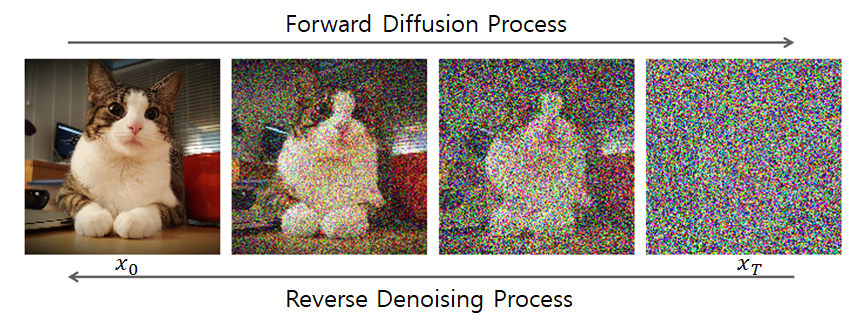
\includegraphics[width=\textwidth]{figure/diffusionModel}
    \caption{Schema di un modello di diffusione: nel processo forward si aggiunge rumore progressivamente a un’immagine, mentre nel processo inverso (reverse diffusion) si parte dal rumore per ricostruire l’immagine originale.}
    \label{fig:diffMod}
\end{figure}

\section{Stable Diffusion}

Una delle implementazioni più rilevanti e ottimizzate dei modelli di diffusione è rappresentata dalla \textbf{Stable Diffusion}. Il suo contributo principale è l’efficienza computazionale, ottenuta spostando il processo di diffusione in uno \textit{spazio latente} compresso, piuttosto che operare direttamente sui pixel dell’immagine. Questo approccio, che ricorda quanto già discusso nei modelli autoencoder, consente di ridurre drasticamente il costo computazionale.

\section{Task dei modelli di diffusione}

Stable Diffusion consente di affrontare molteplici task generativi. Tra i più significativi vi sono:
\begin{itemize}
    \item \texttt{text2img}: generazione di immagini a partire da un prompt testuale;
    \item \texttt{text+image}: generazione o modifica di immagini a partire da un’immagine parziale e un prompt testuale (e.g., image-to-image, inpainting).
\end{itemize}

In entrambi i casi, il modello è composto da tre moduli principali:
\begin{enumerate}
    \item \textbf{Text Encoder}: converte il prompt testuale in un embedding numerico (utilizzando il modello CLIP);
    \item \textbf{Image Information Creator}: un modello U-Net, dotato di uno scheduler, che effettua il processo di denoising nello spazio latente;
    \item \textbf{Image Decoder}: decodifica lo spazio latente nell’immagine finale, tramite un Autoencoder.
\end{enumerate}

\begin{figure}
    \centering
    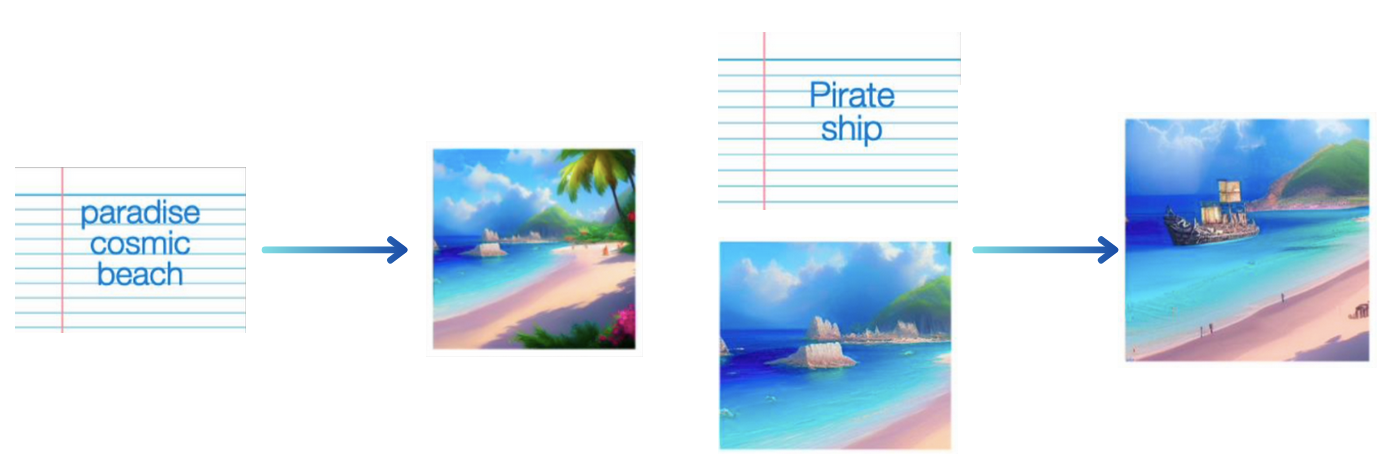
\includegraphics[width=\textwidth]{figure/t2imgAndtextandtext}
    \caption{A sinistra, esempio di task \texttt{text2img}; a destra, task \texttt{text+image} (image-to-image, inpainting).}
    \label{fig:stabDiff}
\end{figure}

\section{Meccanismo di diffusione}

Il processo di diffusione avviene attraverso una sequenza di step successivi. A ogni passo, il modello prende in input un vettore latente e lo aggiorna aggiungendo o rimuovendo informazioni, in funzione del task. Progressivamente, il vettore latente assume una forma sempre più coerente con l’immagine desiderata. Se si visualizzasse il risultato decodificato dopo ciascuno di questi passaggi, si otterrebbe una serie di immagini via via più definite, convergenti verso la versione finale (Figura~\ref{fig:stepDiff}).

\begin{figure}
    \centering
    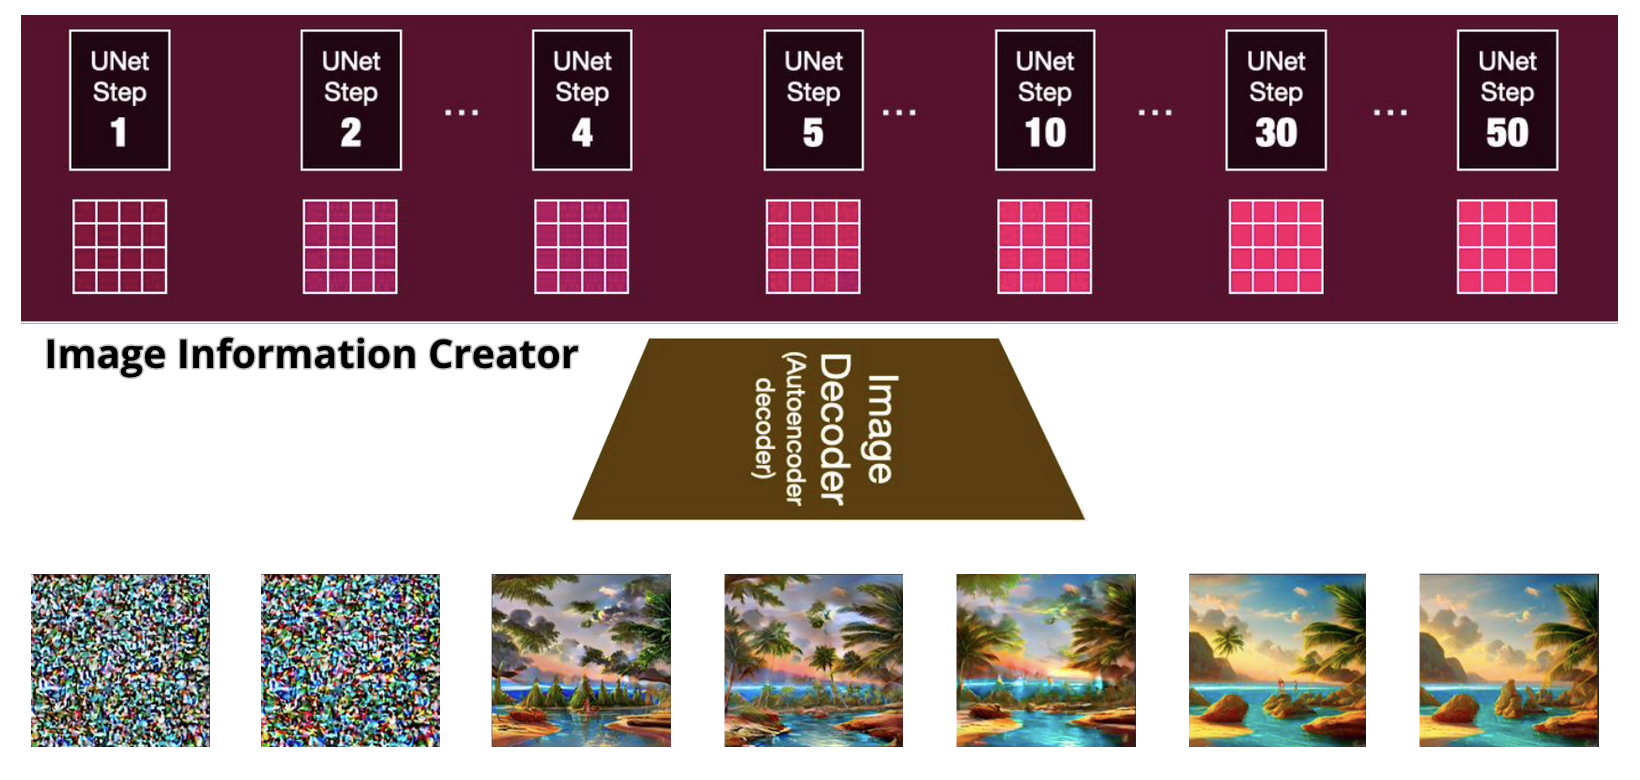
\includegraphics[width=\textwidth]{figure/DiffusionStep.png}
    \caption{Output decodificato progressivamente a ogni step della diffusione inversa.}
    \label{fig:stepDiff}
\end{figure}

\section{Diffusione inversa}

Il processo inverso richiede la conoscenza del quantitativo di rumore aggiunto a un’immagine in ciascuno step. Per questo, si addestra un modello neurale — il \textbf{noise predictor} — a stimare il rumore presente in un’immagine latente. Tale modello è una rete U-Net e viene addestrato come segue:
\begin{enumerate}
    \item Si seleziona un'immagine dal dataset (es. un gatto);
    \item Si genera una quantità casuale di rumore;
    \item Si corrompe l'immagine originale sommando il rumore;
    \item Si addestra il noise predictor a stimare il rumore aggiunto.
\end{enumerate}

Una volta addestrato, il modello può essere utilizzato per il processo di \textit{denoising}: si parte da rumore puro, si stima il rumore presente e lo si sottrae iterativamente. Questo processo, ripetuto più volte, conduce alla generazione di un'immagine coerente (Figura~\ref{fig:revDiff}).
\begin{figure}
    \centering
    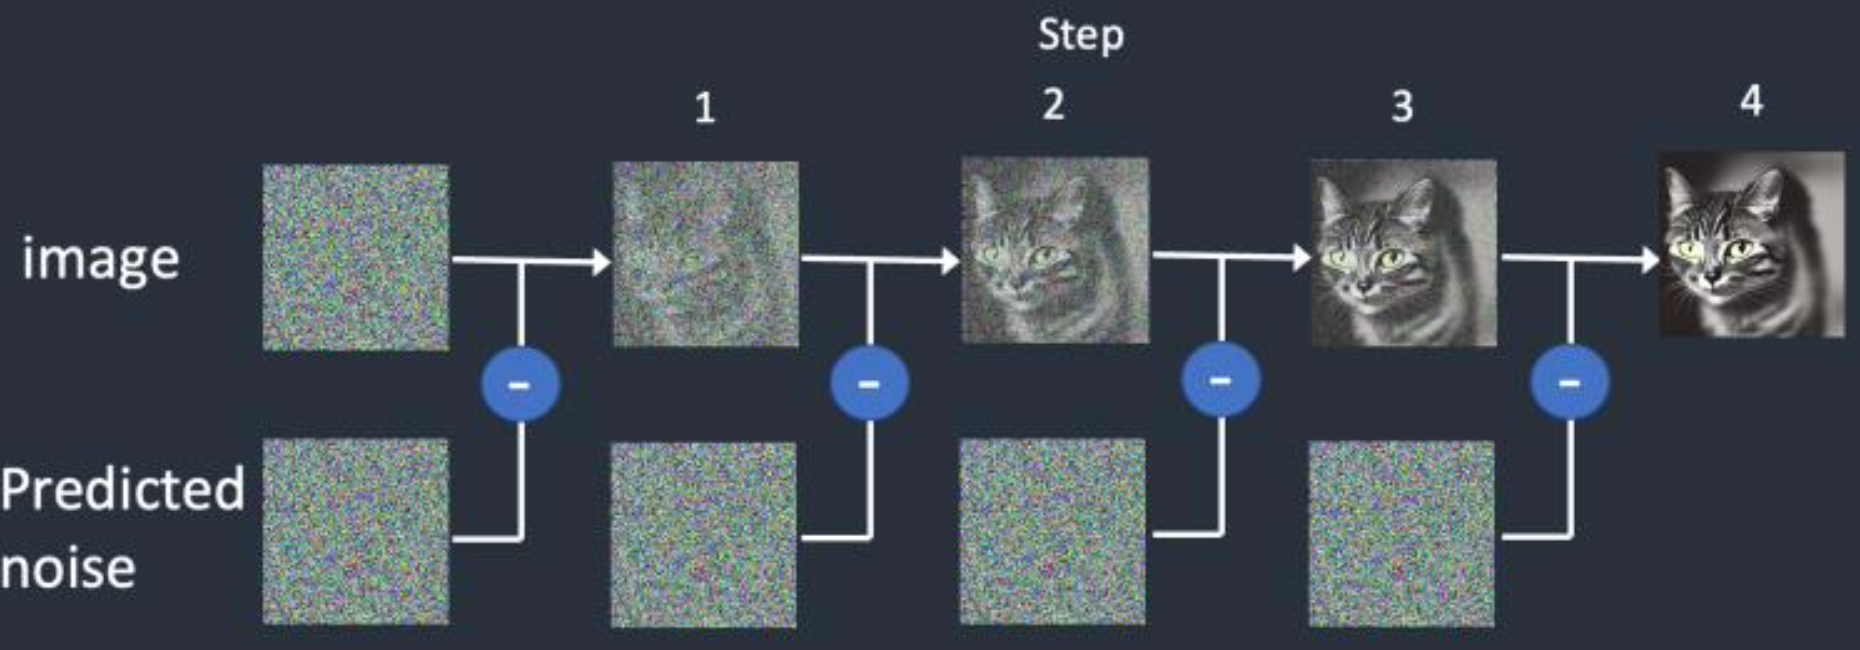
\includegraphics[width=\textwidth]{figure/ReverseDiffusion.png}
    \caption{Esempio di reverse diffusion: il rumore viene rimosso progressivamente fino a ottenere un’immagine pulita.}
    \label{fig:revDiff}
\end{figure}
È importante sottolineare che, in assenza di ulteriori vincoli, la generazione è \textit{incondizionata}, ovvero il contenuto dell'immagine è determinato in modo casuale.

\section{Conditioning}

Per generare immagini coerenti con un prompt testuale, è necessario condizionare il processo di diffusione. Questo avviene introducendo il testo all’interno della pipeline attraverso un \textbf{Text Encoder}, che ne produce un embedding vettoriale. Questo embedding viene poi integrato nel noise predictor tramite meccanismi di \textbf{cross-attention}, permettendo al modello di generare un contenuto visivo coerente con il linguaggio naturale.

\subsection{Cross-Attention}

Il meccanismo di \textbf{cross-attention} consente a una sequenza di essere guidata da un’altra. A differenza della \textit{self-attention}, che confronta una sequenza con sé stessa, la cross-attention confronta una sequenza (es. testo) con un’altra (es. immagine latente). Nel caso di Stable Diffusion:
\begin{itemize}
    \item Il \textbf{Text Encoder CLIP} genera un embedding del prompt;
    \item La \textbf{U-Net} utilizza sia self-attention (per coerenza interna) sia cross-attention (per coerenza col prompt);
    \item Il risultato è un’immagine generata che riflette fedelmente il contenuto testuale.
\end{itemize}

\subsubsection{CLIP}

CLIP combina un encoder per immagini e uno per testi. Durante l’addestramento, dati un’immagine e una descrizione testuale, entrambi vengono trasformati in embedding. Si massimizza poi la \textbf{cosine similarity} tra i due vettori, affinché corrispondano semanticamente. Il processo è iterato e ottimizzato tramite backpropagation.

\subsubsection{Cross-Attention nei Transformer}

Nel contesto dei Transformer, la cross-attention combina due sequenze: una da cui si calcolano le \textit{Key} e \textit{Value}, e una da cui si ottengono le \textit{Query}. Il risultato finale ha la dimensione della sequenza delle Query.
\begin{figure}
    \centering
    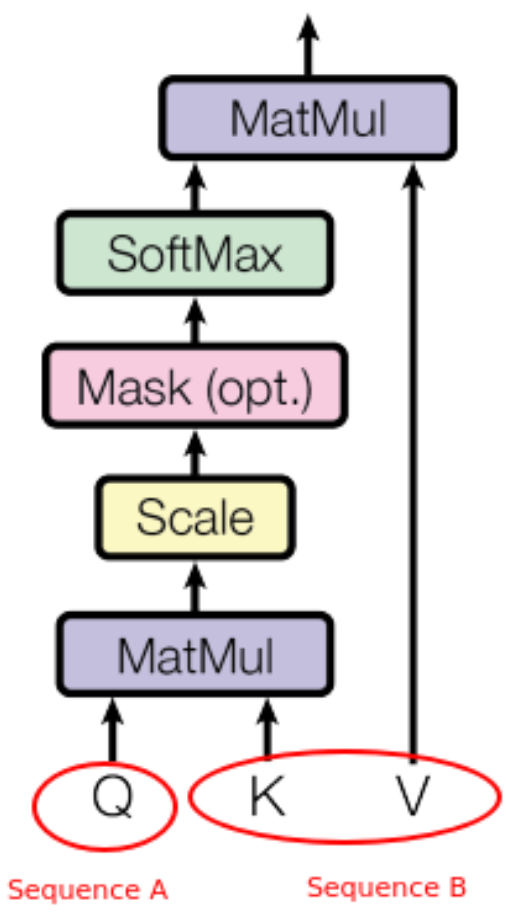
\includegraphics[width=0.25\textwidth]{figure/CrossTrasformer.png}
    \caption{Schema del meccanismo di cross-attention all'interno di un Transformer.}
    \label{fig:crossTrasf}
\end{figure}

\subsubsection{Algoritmo della Cross-Attention}

\begin{enumerate}
    \item Ottenere due sequenze $S_1$ (per Key e Value) e $S_2$ (per Query);
    \item Calcolare $K, V$ da $S_1$;
    \item Calcolare $Q$ da $S_2$;
    \item Calcolare la matrice di attenzione da $Q$ e $K$;
    \item Applicare la matrice di attenzione ai $V$;
    \item L’output ha dimensione pari a $S_2$.
\end{enumerate}

\begin{figure}
    \centering
    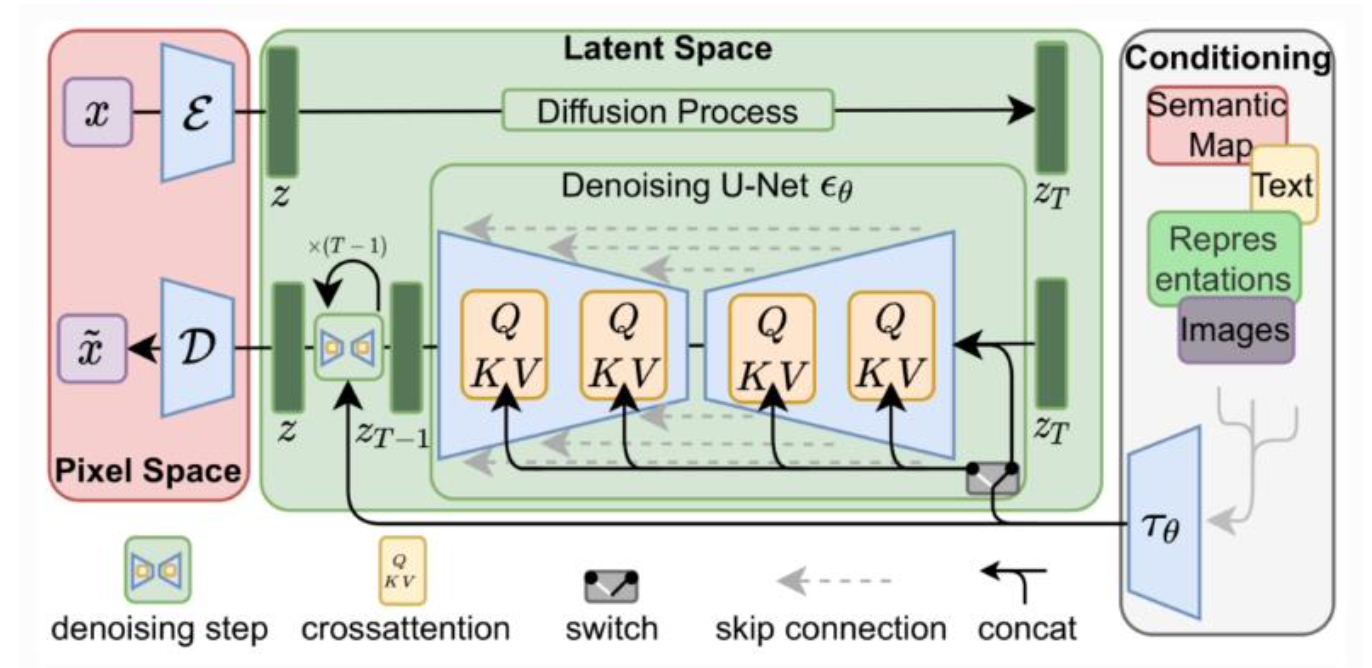
\includegraphics[width=0.7\textwidth]{figure/StableDiffusionArchitecture.png}
    \caption{Architettura completa della Stable Diffusion.}
    \label{fig:StabDiffArch}
\end{figure}

\subsubsection{Cross-Attention nel Perceiver IO}

Il \textbf{Perceiver IO} è un'architettura multimodale in grado di gestire input e output eterogenei. Utilizza la cross-attention per mescolare input multimodali in una rappresentazione latente compatta, permettendo poi la generazione di output flessibili e controllabili.

\section{Ulteriori forme di Conditioning}

Il testo non rappresenta l’unica forma di condizionamento. È possibile condizionare il modello anche tramite immagini, bordi, profondità o pose, ottenendo un controllo più preciso sulla generazione.

\subsection{Image-to-Image}

Nel metodo \textbf{Image-to-Image}, un’immagine grezza e un prompt testuale vengono utilizzati congiuntamente per generare una nuova immagine. Questo approccio, introdotto con SDEdit, segue i seguenti passaggi:

\begin{enumerate}
    \item L’immagine di input viene codificata nello spazio latente;
    \item Viene aggiunto rumore controllato all’immagine latente;
    \item La U-Net predice il rumore tenendo conto anche del prompt;
    \item Il rumore stimato viene sottratto;
    \item Si ripete il processo per più step, fino alla decodifica tramite VAE.
\end{enumerate}

\subsection{Depth-to-Image}

Il metodo \textbf{Depth-to-Image} rappresenta un’evoluzione dell’approccio precedente, introducendo un ulteriore vincolo: la mappa di profondità, stimata con il modello MiDaS. I passaggi sono:

\begin{enumerate}
    \item Codifica dell’immagine nello spazio latente;
    \item Estrazione della mappa di profondità tramite MiDaS;
    \item Aggiunta di rumore controllato;
    \item Predizione del rumore tramite U-Net, condizionata da prompt e profondità;
    \item Sottrazione progressiva del rumore e decodifica finale.
\end{enumerate}

\section{Classifier Guidance e aggiornamenti della Stable Diffusion}

Un'importante estensione dei modelli di diffusione condizionati è l'introduzione del \textbf{Classifier Guidance}, una tecnica che permette di guidare la generazione in modo più deciso verso determinati attributi, agendo come una forza aggiuntiva nel processo di diffusione inversa. In particolare, questo metodo consente di migliorare la fedeltà dell'immagine generata rispetto a una condizione desiderata (es. classe, testo, attributo).

\subsection{Classifier Guidance}

L'idea centrale è semplice: oltre al modello principale di denoising (ad esempio, una U-Net), si introduce un classificatore addestrato per prevedere la classe (o il prompt) associata a un’immagine latente corrotto da rumore. Durante il processo di generazione, si utilizza la \textbf{derivata del logaritmo della probabilità della condizione} rispetto allo stato latente per modificare il processo di denoising, dirigendo l'immagine generata verso un risultato che massimizza la probabilità della condizione desiderata. Formalmente, nel caso di generazione condizionata su una variabile $y$, si desidera campionare da $p(\mathbf{x}_0 | y)$. Per approssimare questa distribuzione, si sfrutta l'identità:
\begin{equation}
    \nabla_x \log p(x_t|y) = \nabla_x \log p(x_t) + \nabla_x \log p(y|x_t)
\end{equation}
dove:
\begin{itemize}
    \item $\mathbf{x}_t$ è lo stato latente corrotto al tempo $t$;
    \item $p(\mathbf{x}_t)$ è la distribuzione incondizionata appresa dal modello di diffusione;
    \item $p(y | \mathbf{x}_t)$ è approssimato tramite un classificatore.
\end{itemize}

Durante la diffusione inversa, si utilizza questo gradiente per modificare lo step di denoising, rafforzando il legame con la condizione desiderata. In pratica, ciò si traduce in una modifica del vettore predetto $\boldsymbol{\epsilon}_\theta(\mathbf{x}_t, t)$ dalla U-Net, aggiungendo una componente proporzionale al gradiente del classificatore:

\begin{equation}
    \epsilon_\theta^{\operatorname{guided}} = \epsilon_\theta(x_t,t) - s \cdot\sigma_t\cdot\nabla_{x_t}\log p(y|x_t)
\end{equation}

dove $s$ è un coefficiente di scala che controlla l’intensità della guida.

\subsection{Classifier-Free Guidance (CFG)}

Un’alternativa estremamente efficace e ampiamente adottata nei modelli moderni (inclusa Stable Diffusion) è il \textbf{Classifier-Free Guidance} (CFG). In questo caso, non si utilizza un classificatore esterno, ma si addestra il modello generativo sia in modalità condizionata che incondizionata. Durante l'inferenza, si combinano le due predizioni per ottenere un controllo sul grado di aderenza al prompt:
\begin{equation}
    \epsilon_\theta^{\operatorname{guided}} = (1 + w)\cdot\epsilon_\theta(x_t,t,y) - w\cdot\epsilon_\theta(x_t,t)
\end{equation}

dove:
\begin{itemize}
    \item $\boldsymbol{\epsilon}_\theta(\mathbf{x}_t, t, y)$ è la predizione condizionata (con prompt);
    \item $\boldsymbol{\epsilon}_\theta(\mathbf{x}_t, t)$ è quella non condizionata (senza prompt);
    \item $w$ è un iperparametro che controlla l'intensità della guida (tipicamente $w \in [1.5, 7.5]$).
\end{itemize}
Questa tecnica consente un'elevata fedeltà al prompt testuale, senza dover addestrare classificatori separati, semplificando l’architettura complessiva.

\subsection{Stable Diffusion 2.0 e versioni successive}

Con la crescita esponenziale della popolarità di Stable Diffusion, sono state rilasciate diverse versioni aggiornate del modello, che introducono migliorie architetturali, prestazionali e qualitative. Le principali innovazioni includono:

\begin{itemize}
    \item \textbf{Addestramento su risoluzioni più elevate} (es. 768x768), per generare immagini di qualità superiore.
    \item \textbf{Nuovi text encoder}, ad esempio OpenCLIP, per una maggiore capacità di comprensione semantica dei prompt.
    \item \textbf{Depth-conditioning} nativamente integrato, per generazioni controllate tramite mappe di profondità.
    \item \textbf{Miglioramenti al VAE decoder}, per ridurre artefatti e aumentare la fedeltà visiva.
    \item \textbf{Introduzione di ControlNet}, un'estensione che permette un controllo fine sulla generazione (e.g., pose, edge, scribble, depth).
\end{itemize}

Stable Diffusion 2.x è diventato un punto di riferimento per la generazione di immagini controllata, aprendo la strada a numerose applicazioni in ambito artistico, pubblicitario, scientifico e industriale.

\section*{Approfondimenti}

\subsubsection*{DDPM (Denoising Diffusion Probabilistic Models)}

I \textbf{DDPM} rappresentano il framework classico dei modelli di diffusione, introdotti da Ho et al. (2020)~\cite{ho2020denoising}. Il processo è modellato come una catena Markoviana di lunghezza $T$, con una forward process che aggiunge rumore gaussianamente e una reverse process approssimata da una rete neurale. Il modello apprende a predire il rumore $\boldsymbol{\epsilon}$ iniettato in $\mathbf{x}_t$:
\begin{equation}
    \mathcal{L_{\operatorname{simple}}} = \mathbb{E}_{t,x_{0},\epsilon}[\|\epsilon - \epsilon_\theta(x_t,t)\|^2]
\end{equation}

Pur offrendo alta qualità, il sampling è lento (richiede centinaia di passaggi).

\subsubsection*{DDIM (Denoising Diffusion Implicit Models)}

Proposto da Song et al. (2021)~\cite{song2021score}, \textbf{DDIM} permette un processo di campionamento deterministico (non stocastico), più rapido ed efficiente. Invece di ricampionare il rumore a ogni step, l'algoritmo definisce una traiettoria implicita nell’input space:
\begin{equation}
    x_{t-1} = \sqrt{\alpha_{t-1}}\cdot x_0 + \sqrt{1-\alpha_{t-1}}\cdot\epsilon_t
\end{equation}

DDIM consente di ridurre il numero di step di generazione (es. da 1000 a 50) senza perdita significativa di qualità.

\subsubsection*{Score-based Generative Models}

Questi modelli, sviluppati in parallelo ai DDPM, si fondano sull’apprendimento dello \textbf{score function} $\nabla_{\mathbf{x}} \log p(\mathbf{x}_t)$, sfruttando tecniche di Stochastic Differential Equations (SDEs). Le score functions vengono apprese a diversi livelli di rumore, e successivamente usate in una reverse SDE per il sampling. La connessione tra questi modelli e i DDPM è stata formalizzata, rendendoli due facce della stessa medaglia: i DDPM sono una discretizzazione specifica di un processo continuo definito dalle SDE.

\subsection*{ControlNet: Controllo strutturato nella generazione}

\textbf{ControlNet} è un'estensione di Stable Diffusion che consente di aggiungere forti vincoli spaziali o semantici durante la generazione di immagini, preservando fedelmente la struttura in input.

\subsubsection*{Motivazione}

La generazione condizionata solo sul testo può risultare ambigua o imprecisa rispetto a vincoli geometrici desiderati (pose, silhouette, contorni, ecc.). ControlNet introduce un secondo input (es. mappa di pose, bordi Canny, depth map), utilizzato per controllare la generazione a livello strutturale.

\subsubsection*{Architettura}

ControlNet replica la U-Net di Stable Diffusion, inizializzandola con i pesi pre-addestrati, ma aggiunge dei \textbf{moduli di controllo} (ad es. convolutioni residue) che elaborano l’input strutturale. Questi moduli sono inizialmente disattivati (zero-conv) e vengono addestrati separatamente. Durante il training, il modello apprende come combinare la guida testuale (prompt) e quella strutturale, garantendo coerenza visiva e semantica.

\subsubsection*{Tipologie di controllo supportate}

ControlNet supporta diverse modalità di conditioning:

\begin{itemize}
    \item \textbf{Pose estimation (OpenPose)}: genera persone in pose specifiche.
    \item \textbf{Canny edges}: preserva bordi di oggetti o silhouette.
    \item \textbf{Scribble / Sketch}: permette agli utenti di disegnare forme rudimentali.
    \item \textbf{Depth maps}: rispetta la disposizione spaziale degli oggetti.
    \item \textbf{Normal maps}: per superfici e orientamenti 3D.
\end{itemize}

Questa flessibilità rende ControlNet uno strumento potente per applicazioni artistiche, design, fashion, architettura e prototipazione visiva.

\subsection*{Modelli a confronto}

\begin{sidewaystable}[htbp]
    \centering
    \caption{Confronto tra principali modelli di generazione di immagini}
    \begin{tabularx}{\textwidth}{|l|X|X|X|X|}
    \hline
    \textbf{Caratteristica} & \textbf{Stable Diffusion} & \textbf{DALL·E 2} & \textbf{Midjourney} & \textbf{Imagen} \\
    \hline
    \textbf{Architettura} & Diffusione latente (VAE + U-Net + CLIP) & Diffusione con VQGAN e CLIP & Proprietaria (non pubblicata) & Diffusione pura + T5 encoder \\
    \hline
    \textbf{Accessibilità} & Open source, estendibile & Accesso tramite API OpenAI & Solo via Discord (chiuso) & Non disponibile al pubblico \\
    \hline
    \textbf{Controllabilità} & Alta: ControlNet, CFG, img2img & Limitata & Bassa, prompt tuning empirico & Alta, ma solo testata internamente \\
    \hline
    \textbf{Qualità visiva} & Molto alta (variabile con CFG) & Alta, dettagli precisi & Alta, stile molto curato & Eccellente, fotorealistico \\
    \hline
    \textbf{Customizzazione} & Altissima (plugin, estensioni, modelli LoRA) & Limitata & Nessuna & Nessuna \\
    \hline
    \textbf{Prompt understanding} & Buono (dipende dal modello CLIP) & Ottimo & Medio-alto & Eccellente (T5 encoder) \\
    \hline
    \textbf{Uso offline} & Sì (tutto in locale) & No & No & No \\
    \hline
\end{tabularx}
\end{sidewaystable}


\begin{Osservazione}
    \textbf{Stable Diffusion} è la soluzione preferita per chi desidera pieno controllo, estensibilità e utilizzo locale. Supporta l’intero ecosistema open-source, inclusi modelli LoRA, ControlNet, DreamBooth, ecc.
\end{Osservazione}
\begin{Osservazione}
    \textbf{DALL·E 2} è adatto a chi cerca semplicità d’uso e buone prestazioni, ma con meno flessibilità.
\end{Osservazione}
\begin{Osservazione}
    \textbf{Midjourney} produce risultati artisticamente curati e stilizzati, ma non offre controllo diretto sulla struttura.
\end{Osservazione}
\begin{Osservazione}
    \textbf{Imagen}, pur dimostrando risultati eccezionali nei paper, non è accessibile pubblicamente per motivi di sicurezza e bias.
\end{Osservazione}

\subsection*{Prompt Engineering}

Prompt ben progettati sono essenziali per ottenere immagini coerenti e di qualità. Un prompt efficace include:

\begin{itemize}
    \item \textbf{Soggetto primario}: "a futuristic city skyline"
    \item \textbf{Modificatori visivi}: "at night, with neon lights"
    \item \textbf{Stile}: "cyberpunk, digital art, trending on ArtStation"
    \item \textbf{Fotografia}: "wide-angle, bokeh, depth of field"
    \item \textbf{Compositing}: "symmetrical composition, ultra-detailed"
\end{itemize}

\subsubsection*{Prompt negativo}

Stable Diffusion supporta anche \textbf{prompt negativi}, usati per escludere elementi indesiderati:

\begin{quote}[scale=0.9]
    \texttt{--negative\_prompt="blurry, low resolution, bad anatomy, extra limbs, disfigured"}
\end{quote}

Questi aiutano a ridurre artefatti e risultati indesiderati.

\subsubsection*{Prompt chaining e combinazioni}

Tecniche avanzate includono:
\begin{itemize}
    \item \textbf{Prompt chaining}: usare l’immagine generata da un prompt come base per il successivo (img2img).
    \item \textbf{Attention weighting}: parentesi per controllare l'importanza di certe parole: \texttt{(cat:1.3)}, \texttt{[tree:0.5]}.
    \item \textbf{Multiple subjects}: separati da "AND" o virgole per composizioni complesse.
\end{itemize}

\subsubsection*{Token embedding personalizzati}

È possibile introdurre token personalizzati (es. \texttt{<sks style>}, \texttt{<johndoe face>}) associati a concetti specifici via fine-tuning o DreamBooth, utili in contesti professionali (moda, branding, VFX).